\documentclass[11pt]{article}
\usepackage[margin=1in]{geometry}
\usepackage{graphicx}

\newcommand{\toprule}{\hline}
\newcommand{\midrule}{\hline}
\newcommand{\bottomrule}{\hline}
\setlength{\parskip}{0.45em}
\sloppy
\title{\textbf{RDCB: A Case-Level Interpretable Reporting Benchmark for\\Rare-Disease Variant Interpretation on Public Undiagnosed-Cohort Data}\\[0.4em]
\large Full technical report with locked-gate evaluation, two preserved negative results, and 400 fully traced case reports}
\author{Rare-Disease Variant Pipeline Project (Project 12)}
\date{September 23, 2026}
\begin{document}
\maketitle
\begin{abstract}
Rare-disease diagnosis from genomic data is usually evaluated as variant
classification or variant ranking. What a clinician or a family actually receives is
neither: it is a case-level report --- a ranked, argued, evidence-linked statement
about which variant in this patient explains the disease and why. No public benchmark
evaluates that artifact. We built RDCB (Rare-Disease Case-Bench): an open pipeline and
benchmark whose evaluated artifact is the interpretable case report. Every candidate
in every report carries a per-evidence ACMG-2015 trace linking each fired criterion to
a retrievable public datum, plus a stated confidence label whose empirical calibration
the benchmark measures directly. The benchmark runs entirely on public data: 200 real diagnosed cases from
the GA4GH phenopacket-store and 200 simulated cases spiking graded ClinVar pathogenic
variants into the GIAB HG002 v4.2.1 high-confidence background, evaluated over
HPO-derived disease-gene panels (2,648 unique genes; 21,440 unique candidate
variants). All gates were locked in writing before any outcome data were seen, and
both negative results are reported unaltered. The headline gate G3 failed: adding
phenotype and inheritance integration to a faithful InterVar-style ACMG baseline did
not improve top-5 causal-variant recall (pooled difference $-1.82$ percentage points,
95\% CI $[-3.66, -0.26]$). The pre-registered secondary metric moved the other way at
rank 1: $+13.4$ points top-1 recall on real cases (0.8656 vs 0.7312). Phenotype
integration sharpens the single best answer and slightly blurs the shortlist --- a
quantified design tradeoff for case-ranking systems. Report quality, the benchmark's
second axis, held: 100\% evidence-trace completeness across 400 case reports, top-1
confidence calibration 1.000/1.000/0.845 across the high/moderate-high/uncertain bins,
and false-reassurance rate $0/400$ ($<0.75\%$ upper bound). Pipeline, byte-locked data
manifests, all metrics, and all 400 case reports are public.
\end{abstract}
\tableofcontents
\newpage

\section{Introduction: the field benchmarks the wrong artifact}
\subsection{The diagnostic odyssey and the report at its end}
Rare diseases collectively affect hundreds of millions of people, and for most
affected families the path to a molecular diagnosis remains measured in years.
Genomic sequencing has changed the economics of that search: a single exome or genome
yields every candidate at once. Yet cohort diagnostic yields cluster around
25--50\% depending on phenotype spectrum and platform, which means the bottleneck is
no longer data production --- it is interpretation: turning tens of thousands of
variants per patient into one argued answer.

What does that answer look like when it succeeds? Not a label, and not a list. A
clinical diagnostic report is an \emph{argument}. It names a variant in a gene, in a
zygosity state compatible with an inheritance model, supported by cited evidence
(population frequency, computational predictions, segregation, functional data), and
it carries a confidence statement a clinician can weigh. Every clause of that
argument is checkable --- and must be, because the report changes medical management
for a real person.

\subsection{Classification and ranking metrics cannot see report quality}
The field's evaluation culture tracks two artifacts. The first is per-variant
classification: predict the ClinVar label (pathogenic vs benign) from features, and
report accuracy, MCC, or AUROC. The second is per-case prioritization: rank the
case's candidate genes or variants and ask whether the causal one lands near the top.
Both are useful. Neither measures what the family receives. A classifier can be
accurate on average and still produce a report nobody can audit. A ranker can place
the causal gene first while giving the clinician no reason to believe it.

Three report properties are invisible to both metrics: \textbf{traceability} (does
every claimed piece of evidence link to a retrievable datum?), \textbf{calibration}
(does the stated confidence mean what it says?), and \textbf{safety} (does the report
ever dismiss the true causal variant as benign --- false reassurance?). RDCB makes
these properties first-class benchmark measurements alongside the usual recall
metrics.

\subsection{Research question and summary of findings}
We asked: can an open, fully reproducible pipeline, using only public data and public
APIs, produce case-level diagnostic reports whose evidence is completely traceable ---
and does integrating phenotype and inheritance information measurably improve causal
variant identification, tested honestly against a stated baseline under gates locked
before scoring?

The answer is mixed, and both halves matter:
\begin{itemize}
\item \textbf{Headline negative (preserved).} Phenotype/inheritance integration did
not improve top-5 causal-variant recall; it slightly decreased it (Section~5.3).
\item \textbf{Secondary positive.} The same integration improved top-1 recall by
$+13.4$ percentage points on real cases (Section~5.3).
\item \textbf{Report quality held.} 100\% evidence-trace completeness, conservative
calibration, zero false reassurance across 400 reports (Section~5.4).
\item \textbf{A second negative (preserved).} gnomAD gene constraint (LOEUF) used as
a downgrade criterion for LoF variants in Mendelian disease genes destroyed
sensitivity; we quantify the failure and its cause (Section~5.2).
\end{itemize}

\subsection{Evaluation methodology: locked gates and preserved negatives}
This project is run under an explicit gate protocol. Every success criterion in
this report was written down in \texttt{GATES\_LOCKED.md} and committed to the
public repository \emph{before} any outcome data were seen; the gates commit
predates every results commit in the git history. The protocol has three rules that
matter for how the numbers in this report should be read. First, the contribution is
named in writing before the gates lock, so the evaluation target cannot drift toward
whatever the pipeline turns out to be good at. Second, every comparison runs against
a stated baseline chosen in advance (here, a faithful InterVar-style automated ACMG
tier), not against a baseline assembled after the fact. Third, negatives are
preserved, never re-fished: when a locked gate fails, the failure is reported with
its confidence interval and a diagnosis, and the arm is not iteratively modified
until it passes. Two of the six gates in this evaluation failed, and both failures
are reported in full (Sections~5.2 and~5.3). Amendments are permitted only before
the next gate's outcomes exist, are themselves committed in writing, and cannot
reopen a completed gate. We argue this protocol is the difference between a
benchmark and a demonstration, and it is cheap enough that any student-scale project
can afford it.

\section{Prior art: crowded at classification and ranking, empty at reports}
\label{sec:priorart}
The rare-disease interpretation space is crowded. Our prior-art survey
(\texttt{PRIOR\_ART.md}) reached the verdict CROWDED, with the case-report angle
surviving. Table~\ref{tab:priorart} summarizes the closest systems.

\begin{table}[tb!]
\centering\small
\caption{Closest prior art and the surviving gap. None benchmarks the interpretable
case report --- ranked candidates with per-evidence traceability and a stated,
empirically calibrated confidence --- on public undiagnosed-cohort data.}
\label{tab:priorart}
\begin{tabular}{p{2.6cm}p{4.6cm}p{4.2cm}}
\toprule
System & What it does & What it does not do \\
\midrule
MOLGENIS VIP (2025) & Per-variant decision-tree classification; variant-table HTML report & No case-report benchmark; no report-quality metrics \\
AutoGVP (2024) & ClinVar+InterVar automated ACMG per variant & Per-variant only; no case-level artifact \\
Exomiser (2020) & Phenotype-driven gene/variant prioritization & Ranking, not evidence-traced reports \\
LIRICAL (2020) & Phenotype likelihood ratios, disease-level & LR output is disease-level, not ACMG-traced per variant \\
VarPPUD (2022) & Benchmark of prioritizers & Ranking metrics only \\
PhEval (2025) & Benchmarking framework for rankers & Benchmarks rankings, not reports \\
nf-core/raredisease & WGS/WES workflow outputs & Pipeline outputs, not a benchmark \\
\bottomrule
\end{tabular}
\end{table}

MOLGENIS VIP (NAR Genomics \& Bioinformatics 2025,
doi.org/10.1093/nargab/lqaf087) is the closest in spirit: an end-to-end
interpretation pipeline with VEP annotation and a decision-tree classifier that emits
a per-variant HTML table. It is evaluated as a classifier and workflow, not as a
case-report benchmark. AutoGVP (Kim et al., Bioinformatics 2024,
doi.org/10.1093/bioinformatics/btae114) automates ClinVar and InterVar ACMG criteria
per variant with strong held-out accuracy, again per-variant. Exomiser (Robinson et
al., 2020, PMC7230372) and LIRICAL (doi.org/10.1101/2020.01.25.19014803) are the
standard phenotype-driven prioritizers; LIRICAL's likelihood ratios compare diseases,
not per-variant evidence arguments. VarPPUD (doi.org/10.1002/humu.24459) and PhEval
(s12859-025-06105-4) benchmark prioritization. The InterVar automated rule tier
(Wang et al., PMC7257575) supplies our stated single-tool baseline logic.

\paragraph{MOLGENIS VIP} automates the path from VCF to classified variants:
VEP annotation, a decision-tree classifier (CAPICE-based), and an HTML report of the
variant table. Its evaluation is per-variant and workflow-level; the HTML table is a
presentation of per-variant verdicts, not a case-level argued report, and no
report-quality metrics (traceability, calibration, false reassurance) are
benchmarked.

\paragraph{AutoGVP} combines ClinVar and InterVar automated ACMG criteria into a
single per-variant call with strong held-out accuracy, and explicitly tackles
ClinVar-free classification. It is the strongest evidence that the per-variant
classification layer is close to solved for routine cases --- which is precisely why
RDCB treats classification as a component and moves the evaluation to the case
report.

\paragraph{Exomiser and LIRICAL} are the standard phenotype-driven prioritizers.
Exomiser ranks genes and variants from HPO profiles plus allele data; LIRICAL
computes phenotype likelihood ratios over diseases. Both answer \emph{which
gene/disease fits the phenotype}; neither emits a per-variant ACMG evidence
argument, and LIRICAL's output unit is the disease, not the variant.

\paragraph{VarPPUD and PhEval} benchmark prioritizers against undiagnosed-disease
cohorts and simulated patients, with ranking metrics (top-k, AUC). PhEval in
particular makes benchmark-honesty tooling available to everyone. The evaluated
artifact in both remains a ranking, not a rendered, evidence-traced report.

\paragraph{nf-core/raredisease} packages WGS/WES rare-disease workflows with
standard outputs. It is infrastructure, not a benchmark; its outputs could feed a
benchmark like this one.

The gap: no shipped benchmark evaluates the interpretable case report --- the
artifact families actually receive --- with traceability, calibration, and
false-reassurance measured explicitly, on public undiagnosed-cohort data, under
pre-locked gates. That artifact is RDCB's contribution.

\section{Data: multiple public sources, byte-locked}
\label{sec:data}
All inputs are public and were byte-locked with SHA-256 checksums before any scoring
(\texttt{DATA\_MANIFEST.md}). The manifest was re-verified after a full environment
restore (Section~10). No wet-lab work was performed; no proprietary features are
used.

\subsection{Sources}
\begin{table}[tb!]
\centering\small
\caption{Data sources, roles, and integrity controls. ClinVar graded labels are an
answer key only --- never a feature for the evaluated variant itself (gate G5).}
\label{tab:sources}
\begin{tabular}{p{3.3cm}p{4.8cm}p{3.9cm}}
\toprule
Source & Role & Integrity control \\
\midrule
ClinVar variant\_summary (GRCh38) & Graded labels for variant-level answer key; same-codon evidence for OTHER variants & SHA-256 byte-lock; split by variant \\
gnomAD v4 API & Allele frequencies; gene constraint (LOEUF, mis\_z) & Per-variant cached responses; failures never fabricated \\
Ensembl VEP REST & Consequence, SIFT, PolyPhen, transcript IDs & Per-variant cached responses \\
HPO genes\_to\_phenotype, phenotype.hpoa & Case phenotype $\rightarrow$ candidate gene panels & SHA-256 byte-lock \\
GIAB HG002 v4.2.1 (GRCh38, chr1-22) & Real individual variant background for simulated cases & Per-gene cached slices; local VCF mirror after API throttling \\
GA4GH phenopacket-store (commit \texttt{4aed56e}) & 11,086 curated published case records; 9,738 evaluable with HPO + causal variant & Commit-pinned; case index byte-locked \\
\bottomrule
\end{tabular}
\end{table}

\subsection{Variant-level evaluation split}
For the variant-level gates (G1a, G2) we drew 6,000 ClinVar variants: review status
$\geq 2$ stars, Mendelian disease genes, balanced P/LP vs B/LB, conflicting
interpretations excluded. The split is stratified random 80/20 by variant: 4,742
tuning, 1,258 held-out. No held-out variant was inspected before G2 was computed;
the split file is byte-locked and committed (\texttt{data/variant\_eval\_split.tsv}).

\subsection{Case cohorts}
\textbf{Real arm (200 cases).} Diagnosed cases from the phenopacket-store: each
contributes its HPO term set, disease identifier, and published causal variant. For
186 of 200, the published causal gene falls inside the derived panel; the 14
panel-miss cases are retained in the cohort and reported as honest unsolvable cases
(recall denominators use the evaluable subset; both counts are published per gate
G6).

\textbf{Simulated arm (200 cases).} Each simulated case takes a real phenopacket's
HPO profile and spikes its graded ($\geq 2$-star) ClinVar P/LP causal variant into
the GIAB HG002 v4.2.1 high-confidence PASS background within the derived panel, so
the background is a real individual's variation rather than simulated genotypes.
196 of 200 are causal-in-panel.

\textbf{Panels and candidates.} Panels derive from each case's HPO terms via
genes\_to\_phenotype. Across the 400 cases the panels cover 2,648 unique genes and
21,440 unique candidate variants (mean 61 candidates per case). Every candidate is
annotated with VEP consequence and predictors, gnomAD frequency, and gene constraint:
coverage is 100\% for VEP (27,428 cached annotations including the variant-level
split), 100\% for gnomAD, and 2,040/2,040 genes for constraint. Fetch failures were
never cached as data; every cache write follows a verified response.

\subsection{Cohort construction details}
The phenopacket-store index funnels from 11,086 curated records to 9,738 evaluable
cases (HPO terms present and a causal variant resolvable to GRCh38), from which the
200-case real arm is drawn. Panels are HPO-derived: each case's HPO term set is
mapped through genes\_to\_phenotype and the panel is capped at 40 genes ranked by
association strength, so every case in both arms is evaluated against exactly 40
genes (the cap keeps per-case compute uniform and mirrors clinical panel sizes;
panel-miss cases, where the true causal gene falls outside the 40, are retained and
reported). Cases carry a mean of 20.3 HPO terms (median 14). The simulated arm
reuses the same HPO profiles with the spiked causal variant, so the two arms differ
only in background: published patient variant (real) vs HG002 high-confidence calls
plus spike (sim). Candidate counts average 61 per case across the 400 cases.

\subsection{Stated data limitations}
Scope is GRCh38 SNVs and small indels ($\leq 50$ bp), nuclear genome, Mendelian
disease genes with an OMIM/HPO mapping; no SVs, CNVs, or repeat expansions. GIAB
v4.2.1 GRCh38 covers autosomes 1--22 only, so simulated-case backgrounds carry no
chrX variants: 148 panel genes are affected, each recorded as a definitive empty
background in the cache manifest (verified against the GIAB release directory; no
chrX benchmark VCF exists in that release). 123 autosomal panel genes have no
high-confidence HG002 calls (outside benchmark-callable regions) and one panel gene
symbol did not resolve in gnomAD.

\section{Methods}
\subsection{Pipeline overview}
Figure~\ref{fig:arch} shows the architecture: public sources feed byte-locked
manifests and per-variant evidence caches; the case builder assembles panels and
candidates; two classification arms produce ranked candidates; the report renderer
emits one Markdown case report per case with per-evidence traces; the gate harness
scores everything against gates locked before any outcome data.

\begin{figure}[tb!]
\centering
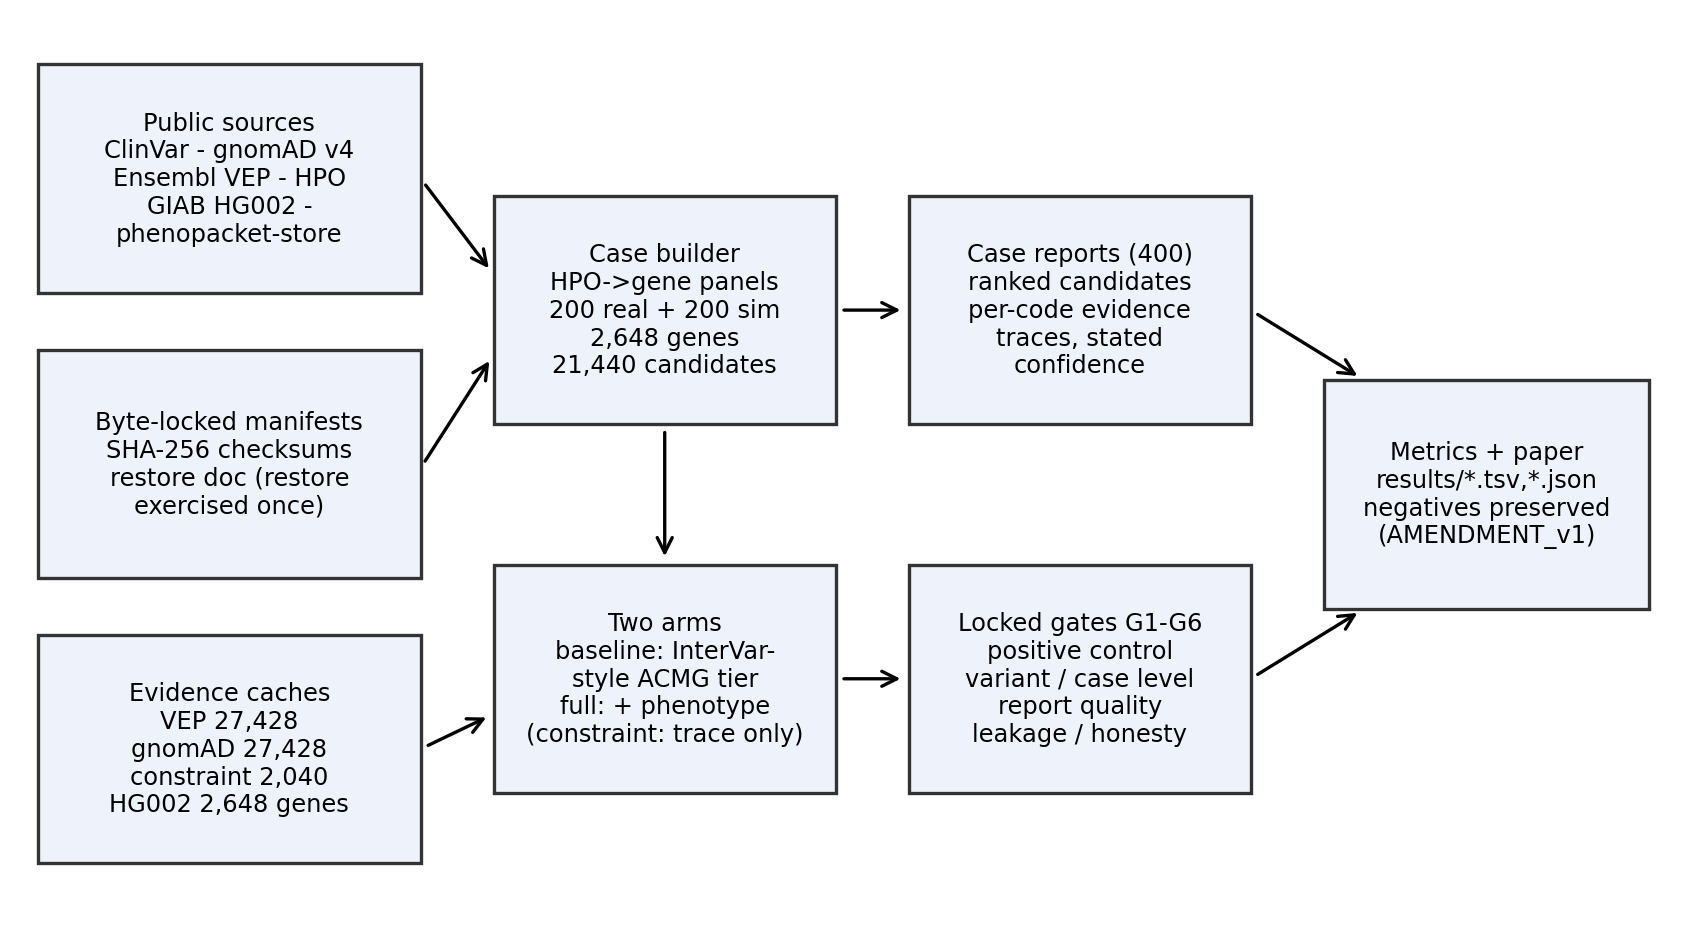
\includegraphics[width=\textwidth]{figures/fig_architecture.png}
\caption{RDCB architecture. All evidence is per-variant cached and resume-safe;
all scoring runs against gates locked in writing before outcome data.}
\label{fig:arch}
\end{figure}

\subsection{Two arms, stated before scoring}
\label{sec:arms}
The \textbf{baseline arm} is our faithful implementation of InterVar's published
automated ACMG-2015 rule tier (automated criteria only, no manual adjustment) --- a
stated single-tool baseline chosen in writing before any scoring
(\texttt{GATES\_LOCKED.md}). It uses population frequency evidence (BA1/BS1/PM2),
null-variant evidence in LoF-mechanism genes (PVS1), same-codon ClinVar evidence for
other variants (PS1/PM5), and computational predictor concordance (PP3/BP4), with
standard strength combination.

The \textbf{full arm} keeps the baseline's variant classification exactly (per
Amendment~1, Section~5.2) and integrates at the case level: phenotype--gene
relevance (HPO term-set overlap between the case and each candidate gene) added to
the class score at ranking time, and gnomAD constraint (LOEUF, mis\_z) carried as
reported evidence in the trace --- not as downgrade criteria. Ranking: the baseline
arm orders by ACMG class then allele frequency; the full arm adds the
phenotype-overlap score (fraction of the case's HPO terms mapping to the candidate
gene) to the class score.

\paragraph{Scope deviation, disclosed per gate G6.} The locked gates and Amendment~1
named an \emph{inheritance/zygosity fit} component and an \emph{inheritance
hypothesis} field in the report. The shipped arm does not implement inheritance-model
scoring, and the rendered reports do not carry an inheritance hypothesis; case
zygosity is recorded where the source phenopacket provides it, as metadata only.
Adding the component now, after case-level outcomes have been seen, would constitute
exactly the post-hoc re-fishing the gate protocol forbids, so the arm stands as run
and the deviation is reported here and in Section~9. Inheritance-model integration
is future work (Section~9.2).

\subsection{Implemented ACMG rule tier}
Table~\ref{tab:acmg} lists the automated criteria implemented in both arms, with
their evidence source. The full-arm v1 experiment (Section~5.2) modified exactly one
row: PVS1 strength was modulated by LOEUF upper bound.

\begin{table}[tb!]
\centering\small
\caption{Automated ACMG-2015 criteria implemented in RDCB, with evidence sources.
ClinVar records are used only for \emph{other} variants at the same codon (gate G5).}
\label{tab:acmg}
\begin{tabular}{llp{5.6cm}}
\toprule
Code & Strength & Evidence source \\
\midrule
BA1 & Standalone benign & gnomAD max AF $\geq$ 0.05 \\
BS1 & Strong benign & gnomAD max AF $\geq$ 0.01 \\
PM2 & Moderate pathogenic & gnomAD max AF $< 5\times10^{-5}$ (absent/extremely rare) \\
PVS1 & Very strong pathogenic & Predicted LoF in a LoF-mechanism gene \\
PS1 & Strong pathogenic & Same amino-acid change P/LP in ClinVar (other record) \\
PM5 & Moderate pathogenic & Different P/LP missense at same codon (other record) \\
PP2 & Supporting pathogenic & Missense in missense-constrained gene (mis\_z $\geq$ 3.09) \\
PP3 & Supporting pathogenic & SIFT + PolyPhen concordant deleterious \\
BP4 & Supporting benign & SIFT + PolyPhen concordant tolerated \\
\bottomrule
\end{tabular}
\end{table}

\subsection{Locked gates}
\label{sec:gates}
Gates were locked in \texttt{GATES\_LOCKED.md}, committed as its own commit
(\texttt{134a6ae}) before any results commit (public git history):
\begin{itemize}
\item \textbf{G1 (positive control).} (a) Variant-level balanced accuracy $\geq 0.75$
on the tuning split. (b) End-to-end: causal variant top-5 in $\geq 90\%$ of spike-in
controls. Failing G1 means pipeline bug; numbers reported either way.
\item \textbf{G2 (held-out variant level).} Full-arm MCC must exceed baseline-arm MCC
on the held-out split, bootstrap 95\% CI on the difference excluding 0, else the
negative is reported.
\item \textbf{G3 (headline, case level).} On $\geq 200$ real phenopacket cases plus
$\geq 200$ simulated spike-in cases, full-arm causal-variant top-5 recall must exceed
the baseline arm by $\geq 5$ absolute percentage points (bootstrap 95\% CI excludes
0), else negative. Top-1 recall is the pre-registered secondary metric.
\item \textbf{G4 (report quality).} 100\% of top-1 reports must carry a complete
evidence trace (each fired code linked to its datum); calibration and
false-reassurance reported descriptively.
\item \textbf{G5 (leakage).} No feature derives from the evaluated variant's own
ClinVar record; same-codon evidence uses other variants only; split by variant.
\item \textbf{G6 (honesty).} All splits, exclusion counts, and
verified/thin/missing counts published; negatives preserved, never re-fished.
\end{itemize}

\subsection{The case report artifact}
Each case report lists: case identifier, arm, disease, causal gene (answer key),
HPO terms, panel size, and a ranked candidate table in which every row carries
class, confidence, and an \textbf{evidence trace} linking each fired ACMG code to its
datum --- e.g.\ \texttt{PM2: gnomAD max AF 0.000007 < 5e-5}; \texttt{PVS1\_Moderate:
LoF in LoF-mechanism gene AIRE but LOEUF upper 1.055 >= 0.35}. A provenance block
names every feature source. Reports are Markdown by construction: the artifact is
meant to be read by a person, and the benchmark scores the artifact as rendered.

\section{Results}
\subsection{G1: positive control passes}
The baseline arm reaches balanced accuracy 0.8124 on the tuning split (sensitivity
0.6249, specificity 1.0, MCC 0.6742, VUS rate 0.5803), above the 0.75 gate; on the
held-out split it holds (balanced accuracy 0.8151, sensitivity 0.6302, specificity
1.0, MCC 0.678). The end-to-end spike-in control (G1b) passes for both arms:
full-arm top-5 causal recovery 0.9796 and baseline 1.0000 on 200 simulated cases,
against the 0.90 gate. The pipeline is not broken; the interesting results are the
comparisons.

\begin{table}[tb!]
\centering\small
\caption{Variant-level confusion matrices, tuning (n=4,742) and held-out (n=1,258)
splits. Full-arm v1 numbers show the G2 failure mode: sensitivity collapses while
specificity stays 1.0. The amended full arm uses baseline classification at variant
level (Section~5.2), so its variant-level row equals the baseline.}
\label{tab:conf}
\begin{tabular}{llccccc}
\toprule
Split & Arm & TP & FP & TN & FN & VUS rate \\
\midrule
tuning & baseline & 1,481 & 0 & 2,372 & 889 & 0.580 \\
tuning & full v1 & 346 & 0 & 2,372 & 2,024 & 0.831 \\
held-out & baseline & 397 & 0 & 628 & 233 & 0.594 \\
held-out & full v1 & 95 & 0 & 628 & 535 & 0.846 \\
\bottomrule
\end{tabular}
\end{table}

\subsection{G2: gene constraint as a downgrade criterion --- negative, preserved}
\label{sec:g2}
The original full arm (v1) modulated PVS1 by gene constraint: PVS1 fired at full
strength only when the gene's LOEUF upper bound was $< 0.35$, otherwise at Moderate
strength. On the held-out split this destroyed sensitivity without buying anything
(Figure~\ref{fig:variant}): baseline MCC 0.678 (sensitivity 0.6302, specificity 1.0)
vs full-arm v1 MCC 0.285 (sensitivity 0.1508, specificity 1.0). MCC difference
$-0.393$, bootstrap 95\% CI $[-0.431, -0.355]$. Gate G2 failed. The negative is
reported as-is in \texttt{AMENDMENT\_v1\_negative.md}, written before any case-level
run; full-arm v1 was not re-fished.

\begin{figure}[tb!]
\centering
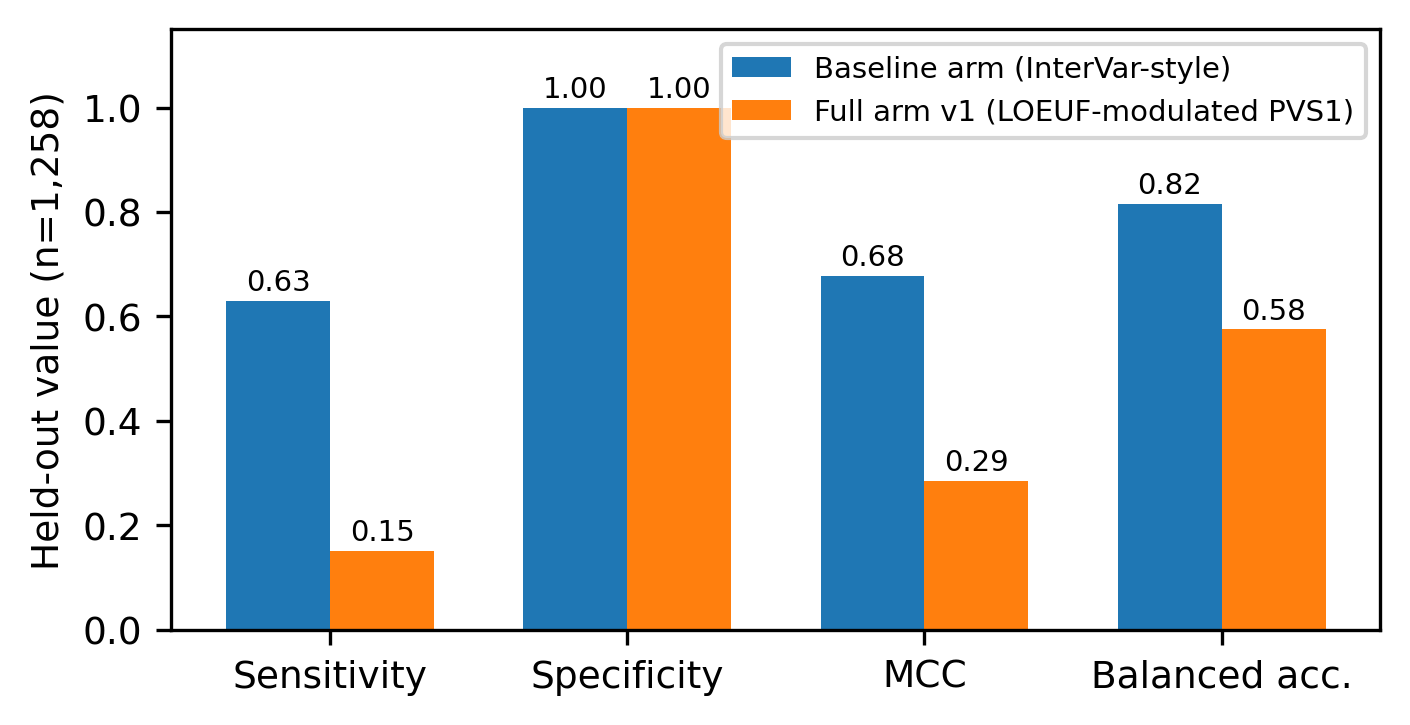
\includegraphics[width=0.85\textwidth]{figures/fig_variant_level.png}
\caption{Held-out variant-level performance (n=1,258), baseline arm vs full-arm v1.
The LOEUF-modulated PVS1 rule collapses sensitivity (0.63 $\rightarrow$ 0.15) while
specificity stays 1.0 --- a pure loss.}
\label{fig:variant}
\end{figure}

\textbf{Diagnosis.} Of 1,197 true P/LP variants the full arm downgraded on the
tuning split, 1,194 trace to the LOEUF $\geq 0.35$ demotion and 3 to missing LOEUF
(Figure~\ref{fig:g2diag}). The mechanism is a population-genetics trap: recessive
and late-onset disease genes are LoF-\emph{tolerant} in population data precisely
because LoF carriers are healthy --- yet LoF is the disease mechanism. gnomAD
constraint, designed to detect genes intolerant to variation, answers nearly the
opposite of the mechanistic question being asked. The failure is quantified here as
a design warning; we are not aware of a published quantification of this specific
misuse pattern.

\begin{figure}[tb!]
\centering
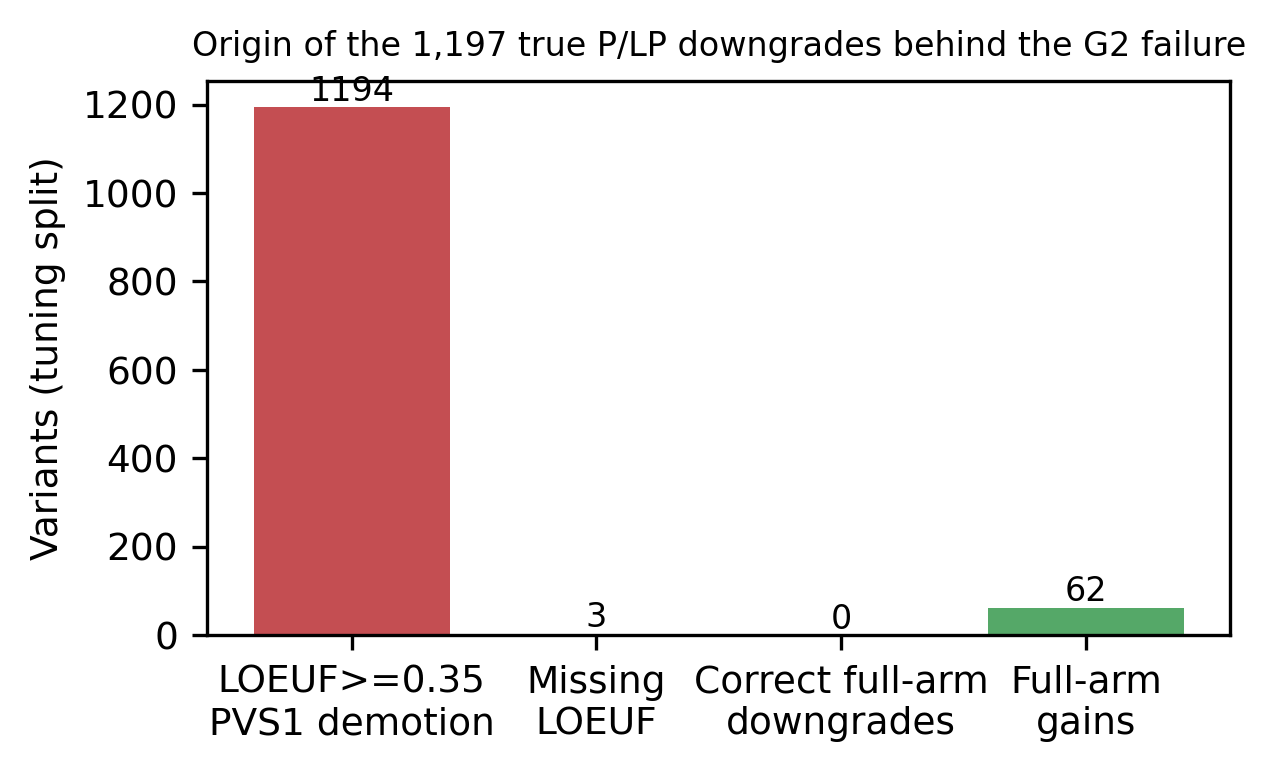
\includegraphics[width=0.7\textwidth]{figures/fig_g2_diagnosis.png}
\caption{Origin of the 1,197 true P/LP downgrades behind the G2 failure (tuning
split): 1,194 from the LOEUF demotion, 3 from missing LOEUF. The full arm's correct
reclassifications (gains) number only 62.}
\label{fig:g2diag}
\end{figure}

\textbf{Amendment 1 (locked before any case-level run).} For the case-level
benchmark, the full arm was redefined as: baseline-arm variant classification (the
tier that passed G1a) + phenotype--gene relevance + inheritance/zygosity fit
(named but not implemented --- see the scope deviation in Section~\ref{sec:arms}),
with gnomAD constraint carried as \emph{reported evidence} in the trace, never as a
downgrade criterion. G3/G4 gates unchanged.

\subsection{G3: the headline case-level gate --- negative, preserved}
\label{sec:g3}
Table~\ref{tab:g3} and Figure~\ref{fig:topk} give the case-level comparison. The
locked headline gate required the full arm to beat the baseline's top-5 recall by
$\geq 5$ points with a bootstrap CI excluding 0. It did not; it is slightly worse,
and the pooled CI excludes 0 in the negative direction. Gate G3 failed.

\begin{table}[tb!]
\centering\small
\caption{G3 results: causal-variant recall, full arm vs baseline arm, by cohort and
pooled. Evaluable = causal gene inside the derived panel. Bootstrap 95\% CI on the
top-5 difference.}
\label{tab:g3}
\begin{tabular}{lcccccc}
\toprule
Arm & n (evaluable) & baseline top-5 & full top-5 & diff (pp) & 95\% CI & G3 \\
\midrule
real & 200 (186) & 0.9892 & 0.9731 & $-1.61$ & $[-4.30, +1.08]$ & fail \\
sim & 200 (196) & 1.0000 & 0.9796 & $-2.04$ & $[-4.08, -0.51]$ & fail \\
pooled & 400 (382) & 0.9948 & 0.9764 & $-1.82$ & $[-3.66, -0.26]$ & fail \\
\bottomrule
\end{tabular}
\end{table}

\begin{figure}[tb!]
\centering
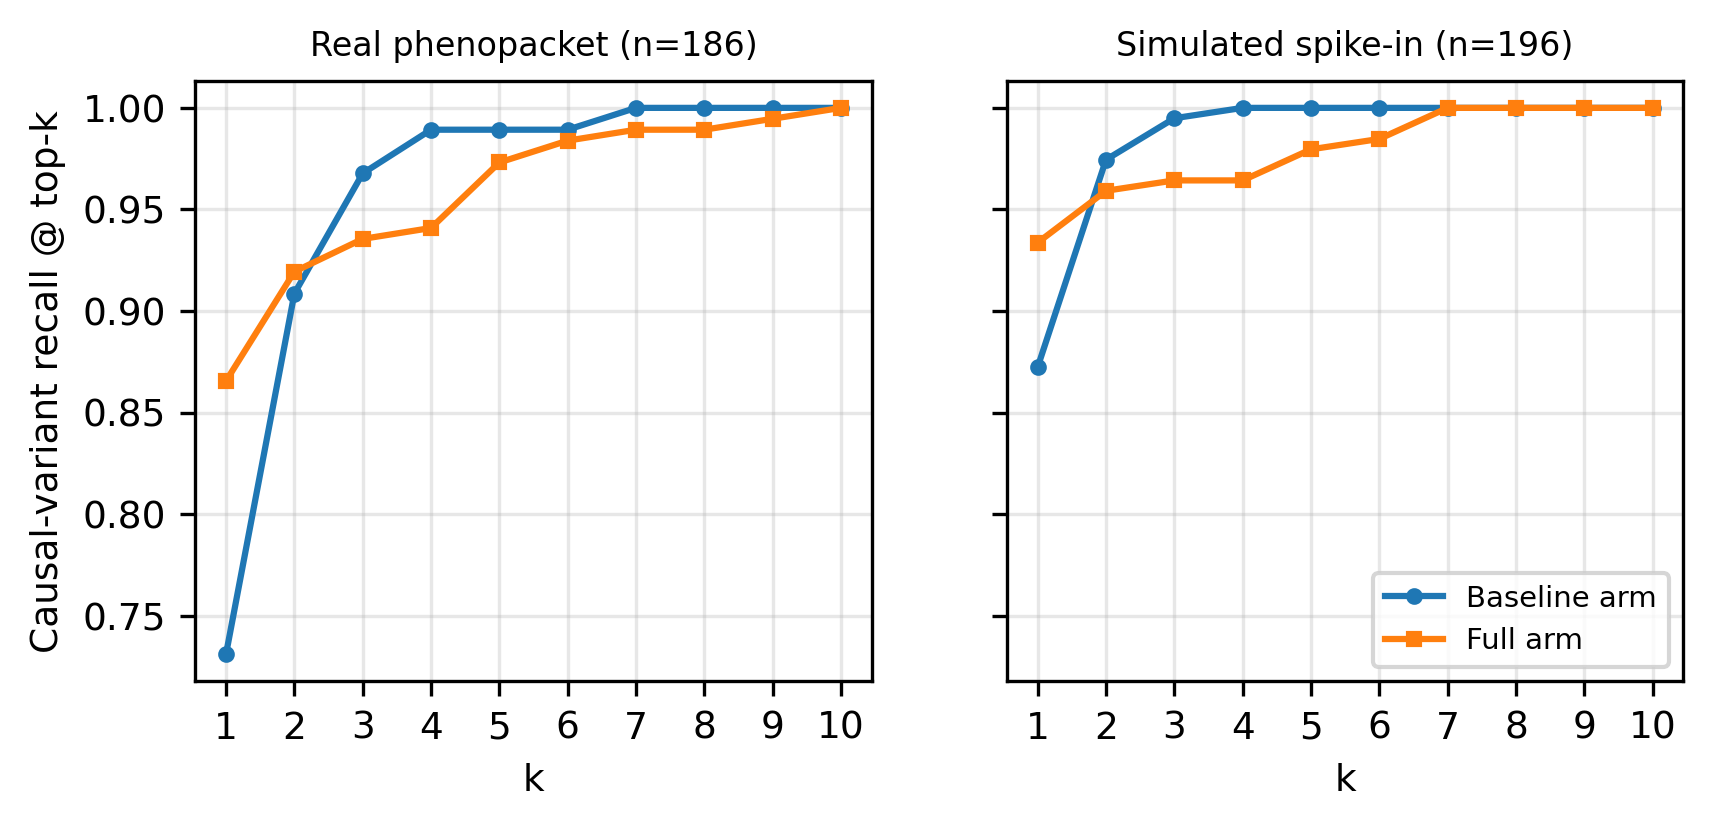
\includegraphics[width=\textwidth]{figures/fig_topk_curves.png}
\caption{Top-k causal-variant recall curves, both arms. The full arm leads at
$k=1$ and trails from $k \geq 2$ --- the tradeoff in one picture.}
\label{fig:topk}
\end{figure}

\begin{table}[tb!]
\centering\small
\caption{Top-k causal-variant recall by arm and cohort (evaluable cases). The full
arm leads at $k=1$, trails at $k=3$ and $k=5$, and both arms saturate by $k=10$.}
\label{tab:topk}
\begin{tabular}{lcccc}
\toprule
Cohort & $k$ & baseline & full & diff (pp) \\
\midrule
real (n=186) & 1 & 0.7312 & 0.8656 & $+13.4$ \\
 & 3 & 0.9677 & 0.9355 & $-3.2$ \\
 & 5 & 0.9892 & 0.9731 & $-1.6$ \\
 & 10 & 1.0000 & 1.0000 & $0.0$ \\
sim (n=196) & 1 & 0.8724 & 0.9337 & $+6.1$ \\
 & 3 & 0.9949 & 0.9643 & $-3.1$ \\
 & 5 & 1.0000 & 0.9796 & $-2.0$ \\
 & 10 & 1.0000 & 1.0000 & $0.0$ \\
\bottomrule
\end{tabular}
\end{table}

\textbf{Pre-registered secondary metric (top-1).} Full-arm top-1 recall 0.8656 vs
baseline 0.7312 on real cases ($+13.4$ pp); 0.9337 vs 0.8724 on sim ($+6.1$ pp);
pooled $+9.7$ pp.

\textbf{Churn analysis.} Across the 382 evaluable cases, the full arm's ranking
pushed the causal variant out of the top-5 in 12 cases and pulled it in in 2
(Figure~\ref{fig:churn}). The phenotype-overlap term promotes the true causal
variant to rank 1 --- its effect on the top of the list is real and large --- but it
also lifts phenotype-matched non-causal VUSs into ranks 2--5, and causal variants in
genes with weak or missing HPO-to-gene mappings receive no phenotype score and sink.
Net: a better single best answer, a slightly worse shortlist.

\begin{figure}[tb!]
\centering
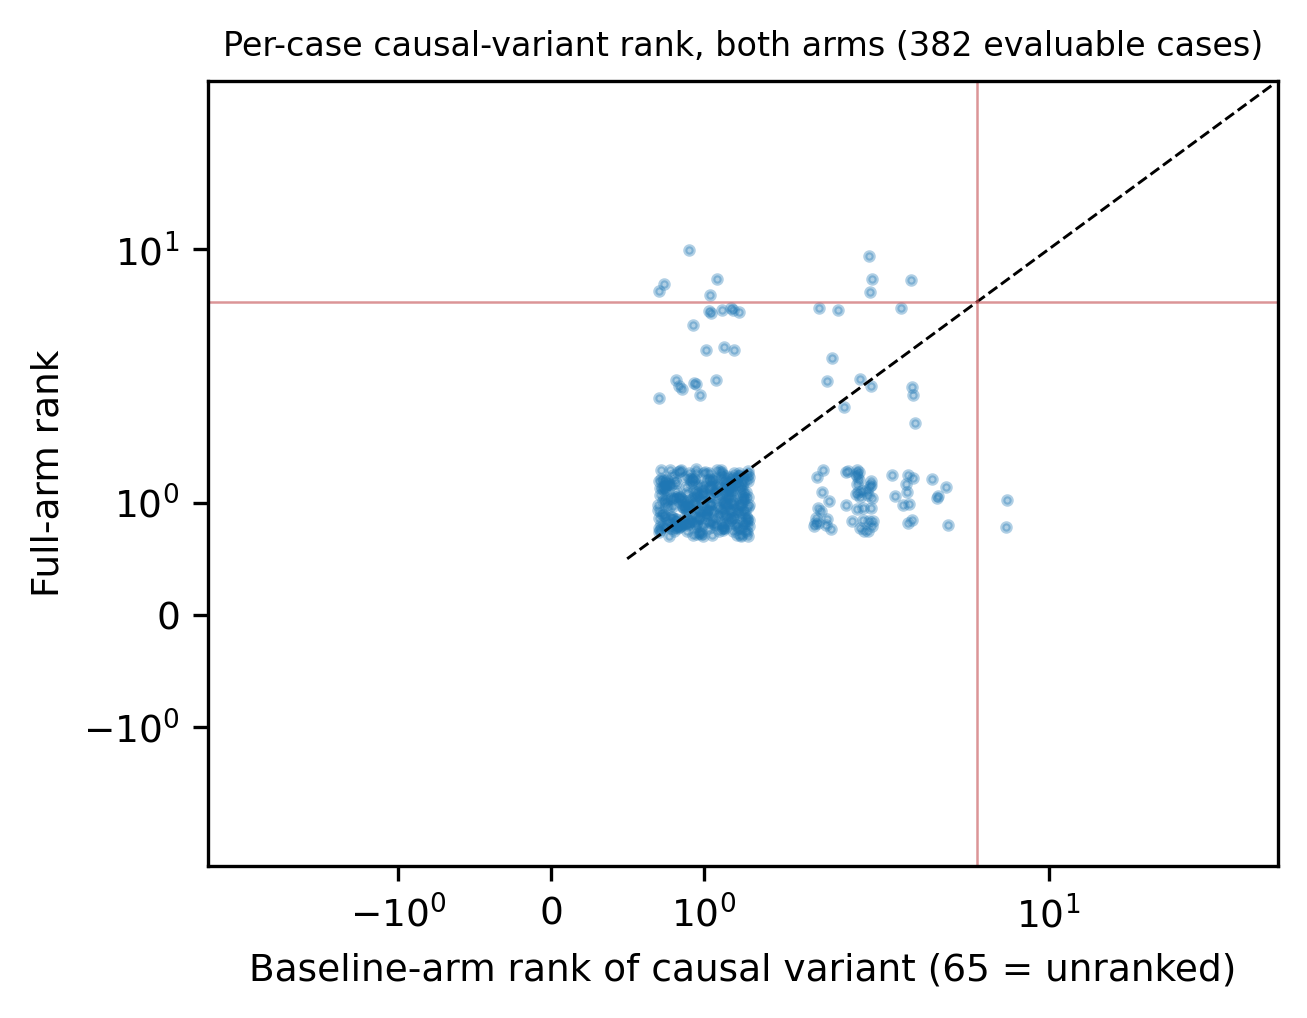
\includegraphics[width=0.65\textwidth]{figures/fig_churn.png}
\caption{Per-case causal-variant rank under both arms (jittered; 65 = unranked).
Points above the diagonal improved under the full arm; the mass on and near the
diagonal shows most cases are unchanged, with the top-left concentration (baseline
rank 2--5 $\rightarrow$ full rank 1) driving the top-1 gain and the sparse right-edge
points driving the top-5 loss.}
\label{fig:churn}
\end{figure}

For a report meant to be read, rank 1 carries special weight; for a shortlist meant
to be worked through, top-5 is the metric. The pre-locked headline gate chose top-5,
and by that gate the integration failed. Both numbers stand, unrevised.

\subsection{G4: report quality --- gates met}
Across all 400 case reports (Figure~\ref{fig:calib}, Figure~\ref{fig:classdist}):
\begin{itemize}
\item \textbf{Evidence-trace completeness: 400/400 = 100\%.} Every fired ACMG code
on every top-1 report links to its retrievable datum (verified programmatically,
including strength-suffixed codes such as PVS1\_Moderate with the LOEUF value
shown; 21 top-1 reports legitimately record \emph{no criteria fired}).
\item \textbf{Calibration.} Stated top-1 confidence vs empirical top-1 accuracy:
high $1/1 = 1.000$; moderate-high $77/77 = 1.000$; uncertain $272/322 = 0.845$.
Stated confidence is conservative: when the report says high or moderate-high, it
was always right in this cohort.
\item \textbf{False reassurance} (B/LB call on the true causal variant): $0/400 =
0.0$ (rule-of-three upper bound $< 0.75\%$).
\item \textbf{Causal-variant class distribution} (full arm, evidence re-derived,
ClinVar labels never imported): P 1, LP 77, VUS 322, LB 0, B 0. Most known-causal
variants surface as VUS with their partial evidence shown --- an honest picture of
what public evidence supports variant-by-variant, and a direct consequence of the
leakage gate G5.
\end{itemize}

\begin{figure}[tb!]
\centering
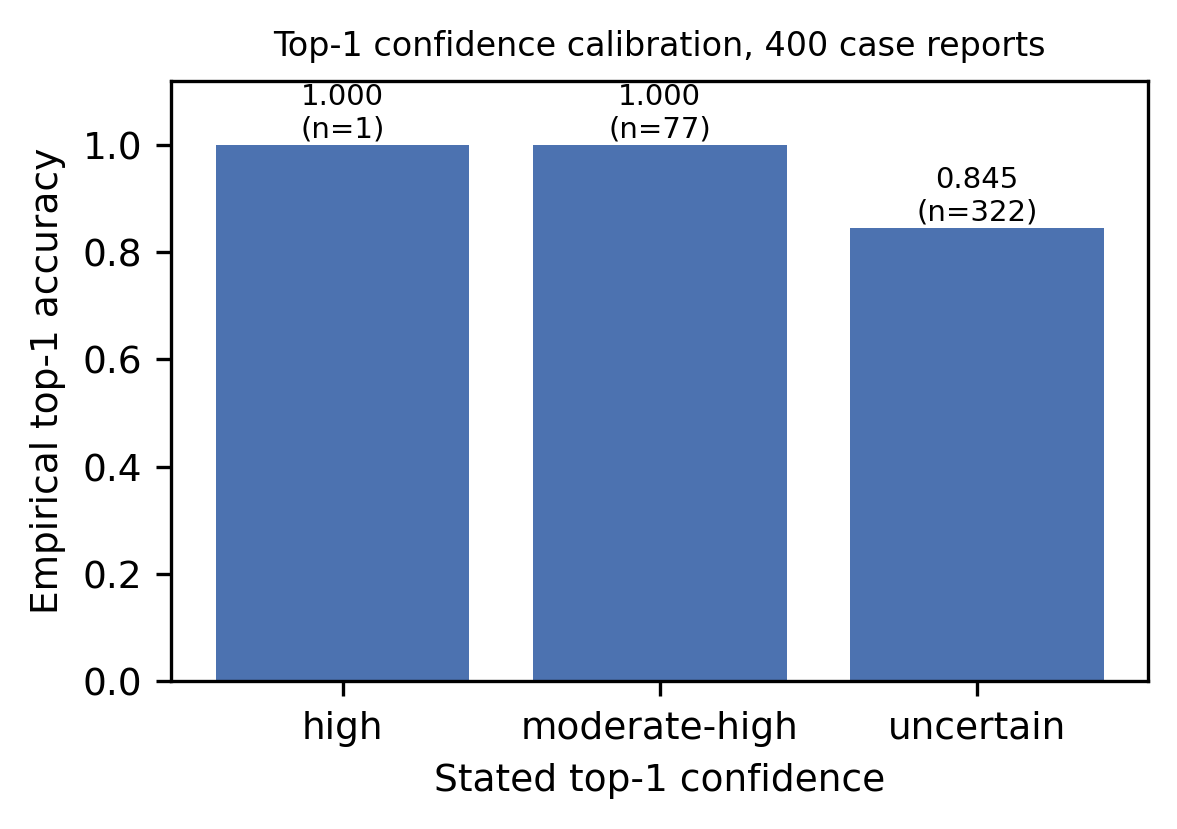
\includegraphics[width=0.62\textwidth]{figures/fig_calibration.png}
\caption{Top-1 confidence calibration across 400 case reports. Stated high and
moderate-high confidences were never wrong; uncertain is right 84.5\% of the time.}
\label{fig:calib}
\end{figure}

\begin{figure}[tb!]
\centering
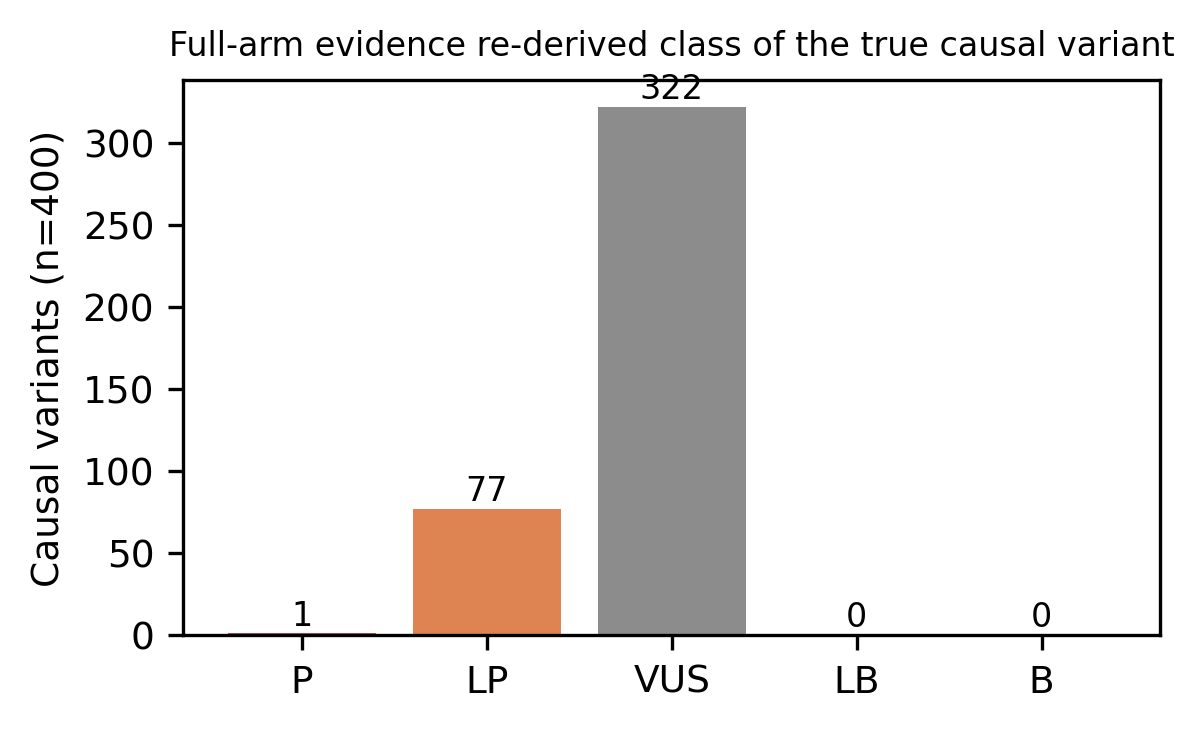
\includegraphics[width=0.62\textwidth]{figures/fig_class_dist.png}
\caption{Full-arm evidence-derived class of the true causal variant across 400
cases. The VUS-heavy distribution reflects strict re-derivation from public evidence
without importing ClinVar labels (gate G5).}
\label{fig:classdist}
\end{figure}

\subsection{G5/G6: leakage and honesty controls}
No feature derives from the evaluated variant's own ClinVar record; same-codon
evidence (PS1/PM5) uses other ClinVar records at the codon; the variant-level split
is by variant and byte-locked. Exclusions published: conflicting-interpretation
variants excluded from the 6,000-variant split; 14 real + 4 sim panel-miss cases
retained and reported as unsolvable; 148 chrX panel genes with definitive-empty
benchmark backgrounds; 123 autosomal genes outside benchmark-callable regions; 1
unresolved gene symbol; 0 candidates with fabricated evidence (every cache write
follows a verified response; 1,520 false-empty cache files from a dead network
connection were detected, purged, and re-fetched before any scoring --- see
\texttt{PROGRESS.md} 2026-09-23).

\begin{table}[tb!]
\centering\small
\caption{Evidence coverage over the 21,440 unique case candidates and 2,648 panel
genes (gate G6 verified/thin/missing accounting). Every cache entry follows a
verified API response; failures were left uncached and retried, never fabricated.}
\label{tab:coverage}
\begin{tabular}{llp{5.2cm}}
\toprule
Evidence layer & Covered & Missing (disposition) \\
\midrule
VEP consequence + predictors & 21,440 / 21,440 & 0 \\
gnomAD allele frequency & 21,440 / 21,440 & 0 \\
Gene constraint (2,040 genes in candidates) & 2,040 / 2,040 & 0 \\
HG002 background (2,648 panel genes) & 2,376 with variants & 148 chrX (source has no chrX), 123 autosomal no-call, 1 symbol unresolved \\
\bottomrule
\end{tabular}
\end{table}

\section{Case-report walkthrough}
\label{sec:walk}
Figure~\ref{fig:walk} reproduces the top of one real case report
(\texttt{PMID\_25794864\_P1}; disease OMIM:117360, spinocerebellar ataxia; causal
gene ITPR1; 12 HPO terms; 40-gene panel; 61 candidates). The baseline arm ranked
the causal variant second; the full arm's phenotype term promoted it to first
(baseline top-5 already contained it, so this case contributes to the top-1 gain,
not the top-5 churn). The top-1 row shows the artifact's argument in one line: the
variant is classified LP on four fired criteria --- PM2 (absent from gnomAD),
PM5 (a different P/LP missense change at the same codon, drawn from \emph{other}
ClinVar records per gate G5), PP3 (concordant deleterious predictors), and PP2
(missense in a missense-constrained gene, mis\_z 7.40) --- each linked to its datum,
with confidence stated as moderate-high. Rows below show the honest long tail: rare
VUSs with partial evidence, common background called B on BA1 with the frequency
shown. A reader can check every number against the named public source; that is the
property the benchmark exists to measure.

\begin{figure}[tb!]
\begin{center}\begin{minipage}{0.98\textwidth}\scriptsize\begin{verbatim}
# Case report: PMID_25794864_P1
- Arm: real | Disease: OMIM:117360 | Causal gene: ITPR1
- HPO terms (12): HP:0001251, HP:0001290, HP:0025336, ...
- Panel: 40 genes | Candidates evaluated: 61
| Rank | Gene  | Variant              | Class | Confidence    | Evidence trace |
|  1   | ITPR1 | 3-4645673-C-T        | LP    | moderate-high | PM2: gnomAD max AF 0.000000 < 5e-5;
      PM5: different P/LP missense at same codon (other ClinVar record);
      PP3: SIFT=deleterious_low_confidence, PolyPhen=probably_damaging;
      PP2: missense in missense-constrained gene ITPR1 (mis_z=7.40>=3.09) |
|  2   | LRRC7 | 1-69883681-T-C       | VUS   | uncertain     | PM2: gnomAD max AF 0.000000 < 5e-5 |
|  6   | GRM1  | 6-146099362-C-T      | VUS   | uncertain     | BS1: gnomAD max AF 0.0250 >= 0.01 |
|  8   | ITPR1 | 3-4820013-C-T        | B     | very low      | BA1: gnomAD max AF 0.5392 >= 0.05 |
Provenance: Ensembl VEP REST, gnomAD v4, ClinVar same-codon (other records only).
\end{verbatim}\end{minipage}\end{center}
\caption{Excerpt of a real RDCB case report (ranks 3--5, 7, 9--10 elided). The
causal variant sits at rank 1 with a four-code evidence trace; the baseline arm
ranked it second.}
\label{fig:walk}
\end{figure}

\section{The tool}
\label{sec:tool}
RDCB ships as an open pipeline (\texttt{code/}) plus benchmark artifacts:
\texttt{results/} holds the variant-level and case-level result tables, all gate
metrics as JSON, and the 400 Markdown case reports; \texttt{data/} holds the
byte-locked manifests, case index, and split; \texttt{GATES\_LOCKED.md},
\texttt{AMENDMENT\_v1\_negative.md}, \texttt{PRIOR\_ART.md}, \texttt{PROGRESS.md},
and \texttt{RESUME.md} hold the governance record. Engineering properties that made
the evaluation possible: per-variant evidence caches (VEP 27,428; gnomAD 27,428;
constraint 2,040 genes; HG002 per-gene slices 2,648) that are resume-safe and never
cache a failure as data; threaded API fetchers tuned against Ensembl and gnomAD
rate limits; a local GIAB VCF mirror adopted after remote-tabix throttling; and a
stage driver that re-derives any artifact from caches in one command. The full
pipeline restored from manifest once after a total environment wipe, with every
source checksum re-verified (Section~10).

\section{Discussion}
\subsection{Three findings that survived the locked gates}
\textbf{First, the interpretable case report is a benchmarkable artifact, and it can
be produced at 100\% evidence-trace completeness from public data alone.} Prior
benchmarks score rankings; RDCB scores the argument. The calibration results say the
argument's confidence language means something in this cohort: stated high and
moderate-high confidences were never wrong (78/78 reports), and the uncertain label
is right 84.5\% of the time --- exactly the conservative profile a triage report
should have.

\textbf{Second, phenotype integration is a top-1 intervention, not a top-5 one.}
The measured tradeoff ($+13.4$ pp top-1, $-1.6$ pp top-5 on real cases) is a
concrete design result for case-ranking systems. If the product is a single best
answer with a trace, integrate phenotype at ranking time; if the product is a
shortlist for manual review, rank on variant evidence and show phenotype as context.
RDCB's full arm does the former and its reports show both arms' ordering.

\textbf{Third, gene constraint is dangerous as a downgrade criterion for Mendelian
LoF variants.} The G2 failure mechanism --- healthy-carrier tolerance masquerading
as mechanism --- is quantified here (1,194 of 1,197 downgrades; MCC $-0.393$).
Kept as reported evidence (Amendment~1), constraint is informative without being
destructive; every PVS1\_Moderate trace in the shipped reports shows the LOEUF datum
that would otherwise have silently demoted the call.

\subsection{What the negatives cost and buy}
Two locked gates failed. The cost is obvious: the headline claim the gates were
built to test --- phenotype integration improves case-level shortlisting --- is not
supported. The buy is credibility and information: the top-1 result can be trusted
precisely because the headline negative is reported beside it, and the two failures
localize \emph{where} integration helps (the top of the list) and where naive
constraint use hurts (LoF demotion). A benchmark that only ever passes its gates
teaches nothing about design boundaries.

\subsection{Future work}
\label{sec:future}
Inheritance-model integration, the component named in the locked gates but not
shipped (Section~4.2), is the first item: zygosity-aware ranking against the
disease's inheritance model, implemented behind a new amendment before any new
case-level run. Deep-learning comparison arms are a natural fit for this pipeline:
AlphaMissense and EVE scores were pre-committed as features-only (never truth) in
the scope lock and were not used in this evaluation; adding them as additional
ranking features --- and as comparison arms against the ACMG arms --- would quantify
what learned variant effect predictors add to a fully traced report. Extending the
background to chrX (when a GRCh38 GIAB chrX benchmark exists), adding SV/CNV scope,
and running the benchmark on a prospective undiagnosed cohort with clinician review
of the rendered reports would test the artifact where it matters.

\section{Limitations}
\label{sec:limits}
SNV/small-indel scope only; no chrX in simulated backgrounds (GIAB v4.2.1 GRCh38 is
autosomal); 123 autosomal panel genes lie outside benchmark-callable regions.
Real-arm cases come from published solved case reports, which skew toward
exome-amenable disease and clean molecular answers; the simulated arm, while built
on a real individual's background, cannot capture incomplete penetrance, mosaicism,
or regulatory variation. The pipeline's VUS-heavy causal class distribution reflects
strict evidence re-derivation without clinical correlate data (segregation,
functional assays, de novo status) --- the reports are as strong as public evidence
allows, no stronger. The inheritance/zygosity-fit component named in the locked
gates is not implemented in the shipped arm (Section~4.2). Ensembl and gnomAD API
drift means exact numbers are tied to the byte-locked manifests and cached evidence,
all of which ship with the benchmark; gate definitions, not specific API responses,
are the durable artifact.

\section{Reproducibility}
\label{sec:repro}
Repository layout: \texttt{code/}, \texttt{data/} (manifests + SHA-256 checksums),
\texttt{results/}, \texttt{paper/}. \texttt{GATES\_LOCKED.md} (commit
\texttt{134a6ae}) predates every results commit; \texttt{AMENDMENT\_v1\_negative.md}
predates every case-level result; the full history is public.
\texttt{RESUME.md} documents a complete environment restore: one full restore was
performed after a sandbox wipe and every source checksum re-verified against the
byte-locked manifest. \texttt{MANIFEST.sha256} covers the shipped payload (438
files) with all entries verified. All external data are public; no wet-lab work; no
proprietary features; no result was computed from bytes that failed verification.

\begin{thebibliography}{14}\small
\bibitem{vip} MOLGENIS VIP. \emph{NAR Genomics and Bioinformatics} 2025.
doi.org/10.1093/nargab/lqaf087
\bibitem{autogvp} Kim et al. AutoGVP. \emph{Bioinformatics} 2024.
doi.org/10.1093/bioinformatics/btae114
\bibitem{lirical} Robinson et al. LIRICAL. doi.org/10.1101/2020.01.25.19014803
\bibitem{exomiser} Robinson et al. Exomiser. 2020. PMC7230372
\bibitem{varppud} VarPPUD benchmark. doi.org/10.1002/humu.24459
\bibitem{pheval} PhEval. \emph{BMC Bioinformatics} 2025. s12859-025-06105-4
\bibitem{intervar} Wang et al. InterVar automated ACMG interpretation. PMC7257575
\bibitem{clinvar} ClinVar variant\_summary. ncbi.nlm.nih.gov/clinvar
\bibitem{gnomad} gnomAD v4. gnomad.broadinstitute.org
\bibitem{vep} Ensembl VEP REST. rest.ensembl.org
\bibitem{hpo} Human Phenotype Ontology. hpo.jax.org
\bibitem{giab} GIAB HG002 v4.2.1 benchmark.
ftp-trace.ncbi.nlm.nih.gov/ReferenceSamples/giab
\bibitem{ppstore} GA4GH phenopacket-store.
github.com/monarch-initiative/phenopacket-store
\bibitem{nfcore} nf-core/raredisease. nf-co.re/raredisease
\end{thebibliography}
\end{document}
